\chapter{Fundamentals of X-Ray Spectrometers}
\label{section: theory}

Since their inception in 1914 \citep{bragg1914x}, x-ray spectrometers 
have 
developed into an indispensable tool for plasma and high-energy 
density matter 
research, where x-rays allow probing into the optically opaque samples \cite{renner2019challenges}. This can be attributed in part 
to the 
unique challenges presented by x-rays and their interaction with 
matter. 
Conventional optics cannot be applied, as no absorption free 
materials are 
available and sufficient reflectivity is only achieved with 
grazing-angle 
incidence, greatly increasing optical aberrations 
\citep{kunze2009introduction}. By necessity, the entire optics of 
the 
spectrometers must therefore be realized using as few components as 
possible. 
In most cases, this limits the components to two; the 
detector and the dispersive element, which spatially separates the 
photons 
according to their energies and in most cases consists of one 
reflecting 
surface, as each new surface reduces the intensity of the x-rays on 
detector. Additionally, the placement of the components in relation to the x-ray source plays a vital role. In light of these limitations, x-ray spectrometers 
are generally designed with the specific experimental scheme and 
goals in mind 
and optimized using ray-tracing codes \citep{renner2019challenges}.

Central to the function of these spectrometers is the dispersive 
element. For 
energies below \eV{250}, gratings are 
generally used, 
owing to their high reflectivity, while for x-rays from 
\eV{250}-\SI{100}{\kilo\electronvolt}, and 
therefore for this work, crystals are more suitable
\citep{renner2019challenges}. The spectral dispersion of the x-rays 
occurs upon 
reflection on the 
dispersive element, where optical path differences between incident 
photons 
lead to interference. If this difference corresponds to multiples of 
the 
photon's wavelength, there is constructive interference, while the 
reflected 
intensity of other wavelengths is suppressed. As the optical path 
difference 
depends on the incident angle, photons are dispersed according to 
wavelength. 
In the case of crystals, this dependence is expressed by Bragg's law 
\citep{yang2011focusing}
\begin{equation}
	n\lambda = 2d_l\sin(\theta),
	\label{Bragg}
\end{equation}
where $n$ is the diffraction order, $\lambda$ the wavelength, $d_l$ 
the lattice 
constant, and $\theta$ the grazing angle.

In this work I will categorize the wide variety of spectrometer 
designs into 
two types; flat crystal and bent crystal spectrometers. Crystals can be 
one-dimensionally 
bent, for example cylindrically, or two-dimensionally, i.e. 
conanically or 
spherically. The type and degree of bending is limited by the 
crystal material 
and available production methods \citep{kunze2009introduction}. 
Typically, flat 
crystal spectrometers 
offer simplicity, ease of build, and more diverse crystal material choice 
with fewer 
defects, while bent crystal spectrometers exhibit the potential for combining dispersion and focusing in one element, yielding 
more 
flexible geometries and potentially high resolution and intensity 
on the detector 
\citep{renner2019challenges,kunze2009introduction}. As a result, 
improved 
signal-to-noise ratios are expected for bent crystal designs, at the 
cost of 
more complicated schemes and potential for crystal defects. 

In this section, I aim to introduce the background and fundamentals 
needed for 
this work. First in section 2.1, the flat crystal design is briefly 
outlined 
and 
explained, also serving as a baseline used to introduce some 
important 
quantities. In section 2.2, bent crystal designs are discussed, 
including an 
overview of the von-Hamos geometry and a more detailed 
explanation of the Focusing Spectrograph with Spatial Resolution (FSSR) 
geometry. Then, in section 2.3, the 
calculations for the dispersion of the spectrometer geometries designed in this work are shown. Lastly, the influences on the resolution are discussed in 
section 2.4.


\section{Flat Crystal Geometries}
\label{section: flat crystal geometry}

An example of a flat crystal spectrometer geometry is shown in fig. 
\ref{BasicSpec}, where the Bragg angle of the central energy, corresponding to 
the ray incident on the center of the detector, is given as 
$\theta_0$ and a Bragg angle of an arbitrary wavelength as $\theta$. For every 
incident angle on the crystal, only one wavelength fulfills the Bragg 
condition, so that the rays are dispersed on the detector with a dispersion 
$d(E)$, where $d$ gives the location of the rays on the detector. 
This 
dispersion equation is essential for processing of the spectra from 
raw data, and is 
therefore to be calculated or, for more elaborate geometries, 
determined using 
ray-tracing procedures.

\begin{figure}[H]
	\centering
	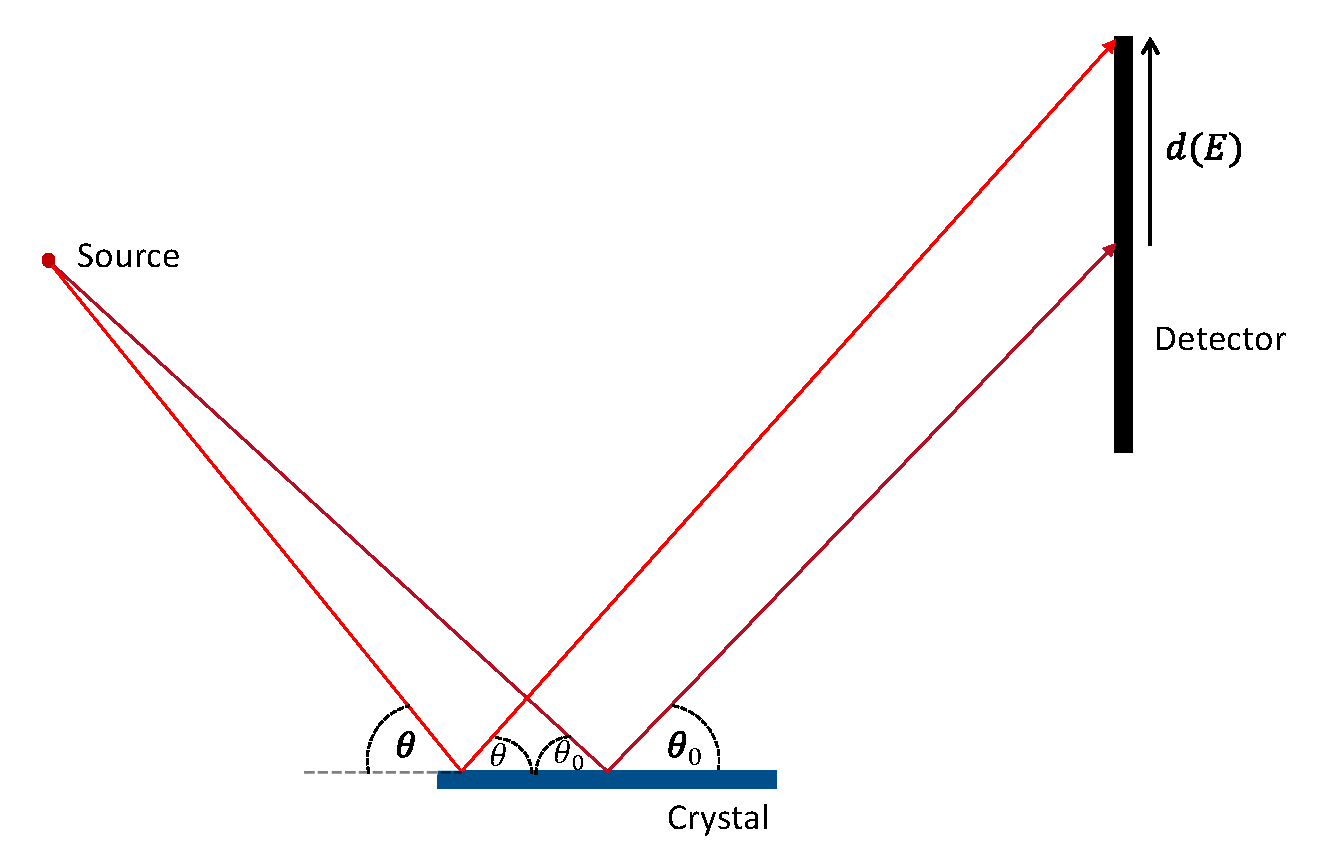
\includegraphics[width = 0.70\textwidth]{Diagrams/Basic_Spectrometer.pdf}
	\caption{Schematic geometry of a spectrometer with a flat crystal.}
	\label{BasicSpec}
\end{figure}

Currently, flat crystal spectrometers are typically eschewed in 
favor of bent 
crystal in the context of high-energy density matter experiments, 
attributed to 
the higher intensity on detector and reduction of source-size 
influences on the 
resolution of bent crystal schemes. If flat crystal schemes are 
used, they 
often come in as compact, easy-to-use mini-spectrometers, mostly 
serving 
supportive roles \citep{renner2019challenges}. Notably, a novel 
type of flat 
crystal spectrometers shows promise, employing two vertically 
orientated plane 
crystals, but is not suitable for this work due to its lower 
collection 
efficiency \citep{renner1999vertical}. Nevertheless, flat 
crystal 
schemes could prove suitable if the experimental scheme covers the 
drawbacks, 
i.e. small source size and intense x-ray source, and a simple 
spectrometer 
scheme with fewer crystal artefacts is desired.

\section{Bent Crystal Geometries}

Bending of the 
crystal allows for higher intensity on the detector, and therefore 
better 
signal-to-noise ratios, as the crystals collect the rays more 
effectively than 
their flat counterparts. Intuitively, this can be understood as more 
surface area of the crystal reflecting light of a certain wavelength 
onto the 
same approximate region on the detector. This comes at the cost of 
possibly 
worsening intrinsic reflection properties of the crystal 
\citep{holzer1998flat}, potentially impacting the inherent resolution due to the 
crystal, 
though the focusing properties of the scheme can 
offset this 
impact \citep{renner2019challenges}. Spherical crystals often entail 
FSSR 
geometries, while cylindrical crystals are applied for von Hamos 
geometries. Both will be handled individually in 
the 
following, with a more detail explanation of the FSSR, which is the geometry used in this work. 

\subsection{Von Hamos Geometry}

The von Hamos geometry is shown schematically in fig 
\ref{SchematicVonHamos}. 
In this case the 
components are placed such that the source and detector lie on the 
cylinder 
axis of the crystal. As a result, all rays emitted from a point 
source with the 
same incident angle on the crystal are focused onto the same point 
on the 
detector, regardless of 
where they are reflected on the circular arc. In effect, the 
geometry leads to 
one dimensional imaging of the source, with the spatial resolution 
along the y 
axis 
and spectral resolution in x direction in fig 
\ref{SchematicVonHamos}. With its 
high collection efficiency and 1-D imaging, this scheme is popular, 
but has the 
drawback of a shallow angle of incidence on the detector and 
sensitivity to 
source broadening in the dispersive direction 
\citep{renner2019challenges}.

\begin{figure}[H]
	\centering
	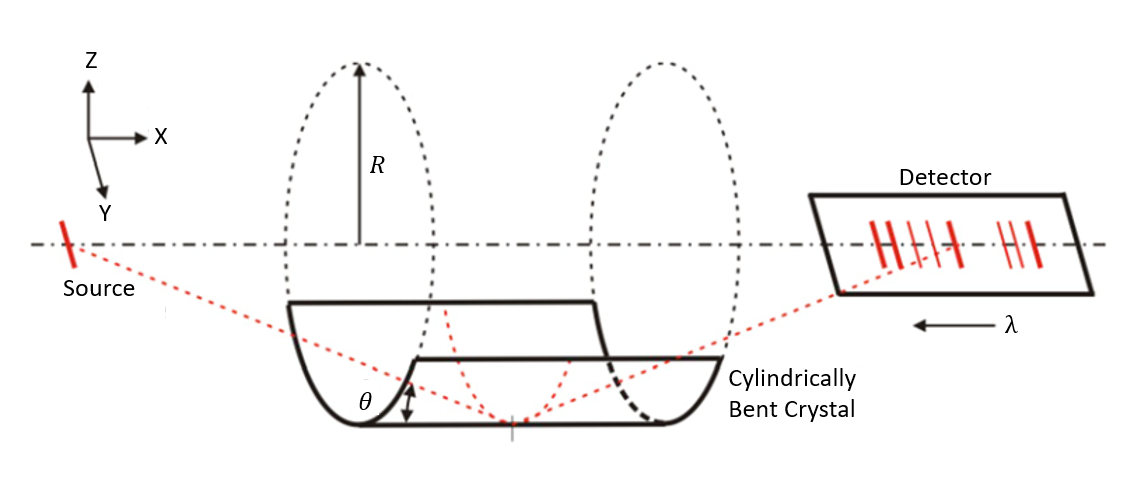
\includegraphics[width = 
	0.90\textwidth]{Diagrams/Schematic_vonHamos.PNG}
	\caption{Schematic representation of a spectrometer of the von 
	Hamos 
	geometry. R represents the crystal curvature radius. 
	\citep{renner2019challenges}}
	\label{SchematicVonHamos}
\end{figure}



\subsection{Focusing Spectrograph with Spatial Resolution} 
\label{SectionTheoryFSSR}

The FSSR has become 
one of the most widely used spectrometer geometries in plasma diagnostics 
\citep{yang2011focusing}, since it offers high luminosity, spectral and spatial 
resolution, and can cover relatively large energy ranges \citep{renner2019challenges}. Its geometry is 
characterized by the 
use of a spherically bent crystal and is commonly separated into two variants, 
the FSSR-1D and 
FSSR-2D, whereby the suffix refers to the dimensions of the source imaging 
\citep{renner2019challenges, blasco2001portable}. Due to its comparable 
simplicity, the function 
of the FSSR-1D will first be described, followed by the FSSR-2D in the final 
paragraph.

Before discussing further, I need to make an aside about the terminology used 
here. When I refer 
to "imaging", I mean imaging in the sense of rays coming from an object plane 
being reflected in such a way that an 
image is formed in the image plane, 
which depends on from where the rays were emitted. This is analogous to what 
occurs for 
lenses and curved mirrors, which is simply the result of 
refraction or reflection on a curved surface. Furthermore I will differentiate 
between 
"mirror imaging" and 
"pinhole imaging", referring to imaging due to mirror curvature in the first 
case and pinholes as in pinhole cameras in the second. On 
the other 
hand, "spectral focusing" refers to the focusing of the rays of the same 
wavelength, but from 
different origins, onto a single point. This is in essence different from 
imaging, since it does 
not inherently form an image, although both cases involve a form of focusing.

A schematic representation of the geometry can be found in fig. 
\ref{3DSchematicFSSR}. To explain the workings of the FSSR-1D, it is 
instructive to define two 
distinct planes, as the properties of the spectrometer change between them. In 
this work they are 
denoted as the dispersive 
plane, containing the direction of dispersion and the circle depicted in fig 
\ref{3DSchematicFSSR}, and the vertical plane, which is perpendicular to the 
dispersive plane and 
includes the detector surface. In the literature these planes are often 
referred to as the 
meridional (dispersive) and sagittal (vertical) planes 
\citep{yang2011focusing,renner2019challenges}. First, I will focus on the 
dispersive plane.


\begin{figure}
	\centering
	\begin{subfigure}[t]{0.58\textwidth}
		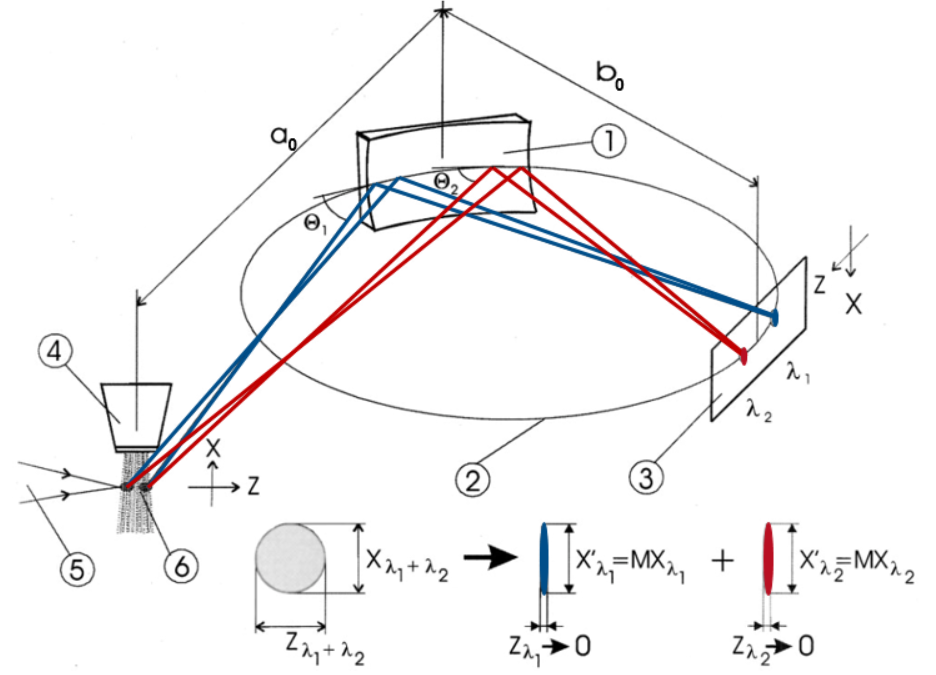
\includegraphics[width=\textwidth]{Diagrams/3DSchematicFSSR.PNG}
		\caption{Schematic depiction of the FSSR-1D spectrometer. (1) 
		Spherically bent crystal, (2) Rowland circle, (3) detector, (4) target 
		material (in the diagram a gas, in this work a foil), 
		(5) laser beam, (6) laser-produced plasma. Additionally the 
		imaging of the source is shown on the bottom, where a 1D-image is 
		formed for each wavelength. \citep{blasco2001portable}}
		\label{3DSchematicFSSR}
	\end{subfigure}%
	\hfill
	\begin{subfigure}[t]{0.38\textwidth}
	\centering
		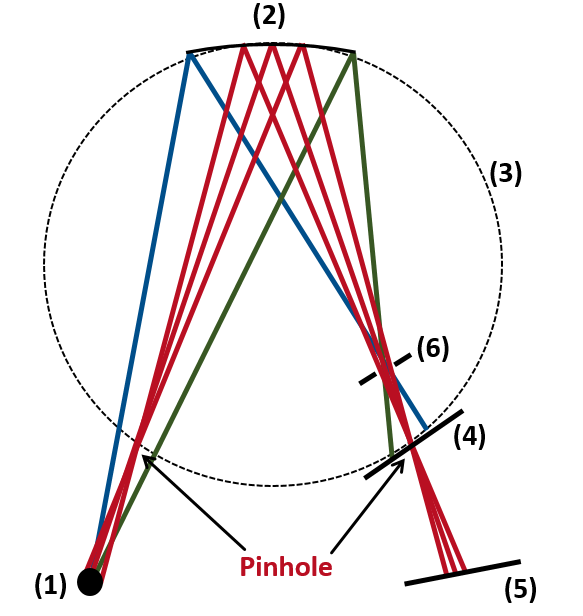
\includegraphics[width=\textwidth]{Diagrams/2D1DFSSR.PNG}
		\caption{Schematic comparison of the FSSR-1D and 2D configurations. (1) 
		Source, (2) 
		spherically bent crystal, (3) Rowland circle, (4) detector in FSSR-1D, 
		(5) detector in 
		FSSR-2D, (6) aperture at polychromatic crossover. Also pictured is the 
		location of the 
		pinhole-like points for the rays of a single 
		wavelength, here in red.}
		\label{FSSRComparison}
	\end{subfigure}
	\caption{FSSR Schemes.}
	\label{FSSRSchemes}
\end{figure}


An important concept to this configuration in the dispersive plane is the Johann 
geometry 
\citep{johann1931erzeugung}, which utilizes the so-called
Rowland circle (RC) (see fig. \ref{FSSRSchemes}), defined as a circle 
tangential to the spherical 
crystal at its midpoint with the radius $R/2$, where $R$ is the radius of the 
crystal 
curvature.  According to this geometry, any ray with a given wavelength that 
passes 
through a certain point on the RC fulfills the Bragg condition everywhere on 
the crystal surface and is focused in first approximation onto 
another point on the RC, mirrored across the crystal curvature pole. All other 
rays of this wavelength, which do not pass through this point, do not fulfill 
Bragg's law anywhere on the crystal and are hence not 
reflected. This effectively results in spectral focusing of the light onto the 
RC independent of where the rays are emitted, as schematically illustrated 
in fig. 
\ref{3DSchematicFSSR}, where the red and blue rays indicate different 
wavelengths. To note here is 
also that placing the detector on the RC is the defining feature of the FSSR-1D 
\citep{monot2002high}.

For both planes, mirror imaging properties are an additional important aspect originating from the spherical bending, comparable to imaging from a concave 
mirror and 
therefore in itself independent of wavelength. There are two focal lengths, one 
for each plane,  
which result from astigmatism due to the off-axis location of the source with 
respect to the 
crystal. The imaging condition, which follows from the mirror equation, in the 
vertical plane is 
\citep{blasco2001portable} 
\begin{equation}
	\frac{1}{a}+\frac{1}{b} = \frac{(2\cos(\alpha))}{R},
	\label{Sfocusing}
\end{equation}
where, for a given ray, the distance between emission point and crystal 
incidence is denoted as 
$a$, the distance between crystal incidence and detector incidence as $b$ and 
the Bragg angle as 
$\theta$, with $\alpha = 
90\degree - \theta$. To achieve the best 
possible spectral resolution and imaging, the source-crystal distance $a_0$, where the 
index 0 refers to the 
central ray, and the crystal-detector distance $b_0$ are chosen 
so that eq. \ref{Sfocusing} is satisfied \citep{blasco2001portable, 
renner2019challenges,faenov1994}. This ensures sharp imaging in the vertical 
plane. It is 
important to note that for the FSSR-1D, there is no imaging on the detector in 
the dispersive 
plane, as the detector lies on the point of spectral focusing. Despite this, 
the mirror imaging in 
the dispersive plane (see \citep{blasco2001portable}) does lead to a 
convergence of rays of 
different wavelengths onto a region between detector and crystal. By placing an 
aperture on this 
region, referred to as the polychromatic crossover (see fig. 
\ref{FSSRComparison}), extraneous 
rays are blocked, reducing the 
background on the detector \citep{renner2019challenges}. Through mirror imaging 
and spectral 
focusing, the FSSR-1D produces a series of 1D, spectrally distinguished images 
on the detector, as 
depicted in the bottom of fig. \ref{3DSchematicFSSR}. 

In the other variant of the FSSR, the FSSR-2D, the detector is placed anywhere 
not on the RC 
\citep{faenov1994}. If the detector and source lie outside of the RC, pinhole 
imaging for each 
wavelength is realized in the dispersive plane. The "pinholes" are a result of 
the spectral 
focusing and are located on the RC as labeled in fig. \ref{FSSRComparison}. A 
good way to imagine 
this is by removing everything inside the RC and bringing the "pinholes" 
together, forming a 
typical pinhole camera setup for each wavelength. Hence 
the magnification in the dispersive direction depends on the 
distance of the source and detector respectively to the RC 
\citep{renner2019challenges}. This pinhole imaging in the dispersive plane, 
along with mirror 
imaging in the vertical plane, results in a series of 2D spectrally selected 
images on the 
detector with different magnifications in each plane \citep{pikuz1995bragg}. In 
general, the 1D 
configuration yields the highest possible spectral resolution, since there is 
minimal overlap of energies due to spectral focusing, while the 2D setup allows 
for 2D 
quasi-monochromatic imaging of the source at the cost of reduced spectral 
resolution \citep{renner2019challenges}. Accordingly, the FSSR-2D setup is 
suitable for use with a 
source that emits a quasi-discrete spectrum, as a continuous spectrum would 
lead to a continuous 
set of 2D-images, leading to very low spectral resolution.




\section{Dispersion Calculation}
\label{section:dispersion calculation}
The dispersion $d(E)$ of x-ray spectrometers shows the relation between a spatial 
coordinate, in this work $d$ as defined in fig. \ref{DispersionDUCK}, and the energies $E$ of the photons. Therefore $d(E)$ 
quantifies where each photon with energy $E$ is expected to land on the 
detector dispersive line for a given spectrometer configuration. Generally 
speaking, an approximately linear dispersion is desirable, since it simplifies 
data processing and ensures an even spread of energies on the detector, so that 
no information is lost due to variable resolution \citep{yang2011focusing}. I 
will calculate the dispersion for the two geometries used in this work, 
namely for the flat crystal geometry found in fig. \ref{BasicSpec} and the 
FSSR as depicted in fig. \ref{FSSRComparison}. 

\subsection{Flat Crystal Geometry}

\begin{figure}[H]
	\centering
	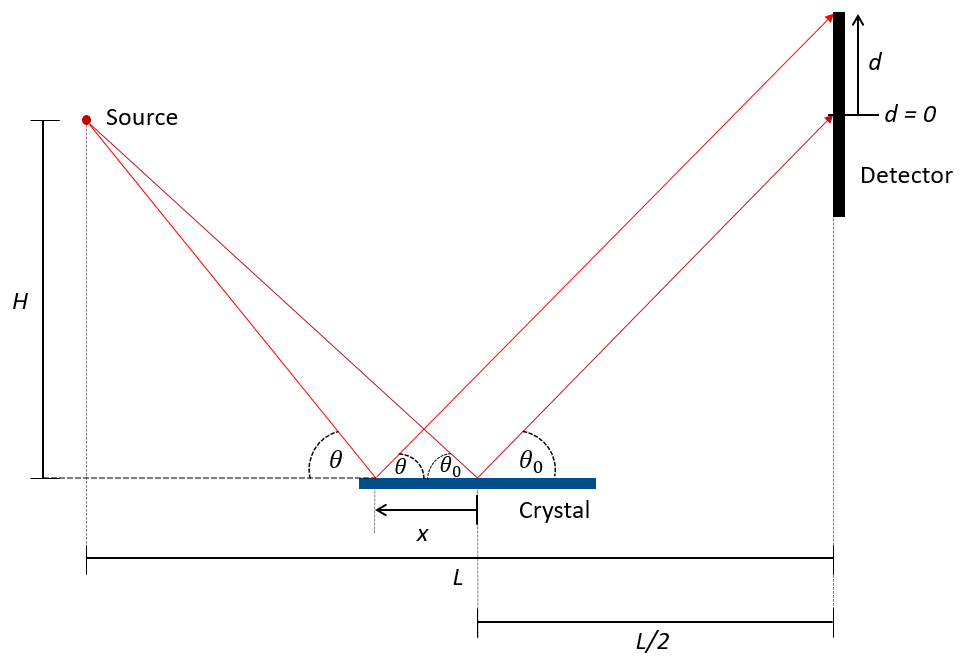
\includegraphics[width=0.8\textwidth]{Diagrams/DUCKDispersionCalc.PNG}
	\caption{Schematic representation of a flat crystal geometry with the 
	detector 
	perpendicular to the crystal surface.  $d$ is 
	defined as lying on the intersection of the dispersive plane and detector 
	surface, with its origin on the location of the central ray, corresponding 
	to $\theta_0$, on the detector. x is the distance between the 
	incident points
	of a given ray and of the central ray on the crystal in the dispersive 
	plane. H is the height of the spectrometer, i.e., the vertical distance 
	from 
	the 
	source to the crystal surface, and L is the length of the 
	spectrometer, i.e., the source-detector distance.}
	\label{DispersionDUCK}
\end{figure}

I will calculate the dispersion for the flat crystal configuration using 
trigonometry and the Bragg condition. The parameters used can be referenced 
from fig. \ref{DispersionDUCK}. From the path of the non-central ray in the 
diagram with the Bragg angle $\theta$, I get the two relations
\begin{subequations}
	\begin{align}
		\tan\theta &= \frac{H+d}{\frac{L}{2} + x} \label{eq:duckdispa} \\
		\tan\theta &= \frac{H}{\frac{L}{2}-x}. \label{eq:duckdispb}
	\end{align}
\end{subequations} 
Setting the right hand sides equal to each other and solving for $x$ yield
\begin{equation}
	x = \frac{L}{2}\cdot\frac{d}{d + 2H}.
\end{equation}
I then plug this into eq. \ref{eq:duckdispa} and simplify, 
which gives
\begin{equation}
\tan\theta = \frac{d}{L} + \frac{H}{\frac{L}{2}}.
\end{equation}
By identifying $\frac{H}{L/2} = \tan\theta_0$ and solving for $d$, I can write
\begin{equation}
d = L(\tan\theta-\tan\theta_0).
\end{equation}
Finally, using Bragg's law (see eq. \ref{Bragg}) and 
\begin{equation}
	\tan\theta = \frac{\sin\theta}{\sqrt{1-\sin^2\theta}} = 
	\frac{1}{\sqrt{1/\sin^2\theta - 1}},
\end{equation}
I receive the dispersion for the flat crystal geometry with detector 
perpendicular to the source
\begin{equation}
d(E) = L\left(\frac{1}{\sqrt{\left(\frac{2d_l}{nhc}\right)^2E^2 - 1}}  - 
\frac{1}{\sqrt{\left(\frac{2d_l}{nhc}\right)^2E_0^2 - 1}}\right),
\label{DispersionCalcDUCK}
\end{equation}
where $E_0$ denotes the energy of the central ray, $h$ the Planck constant and 
$c$ the speed of 
light, which is used in the conversion $\lambda = hc/E$. 
Consequently the dispersion is determined by four parameters in total: $n$, 
$d_l$, $E_0$ and $L$.

\subsection{Focusing Spectrograph with Spatial Resolution}

\begin{figure}[H]
	\centering
	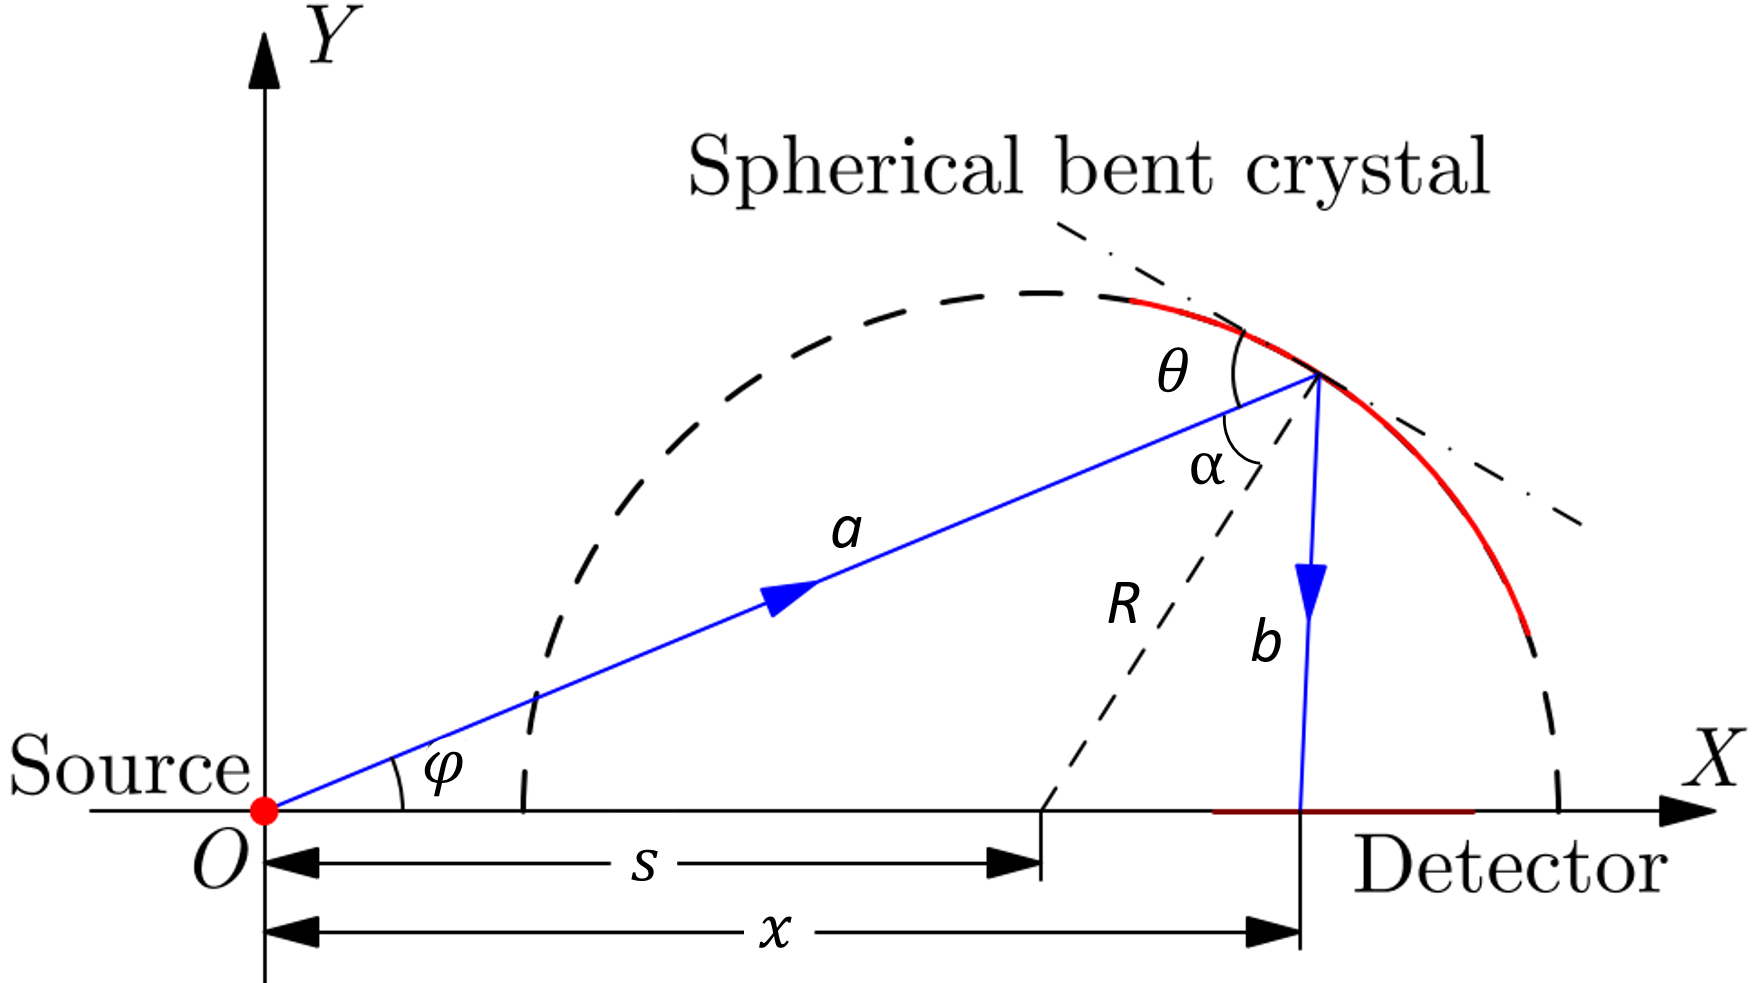
\includegraphics[width=0.8\textwidth]{Diagrams/FSSRDispersionYang.PNG}
	\caption{Geometry of an FSSR spectrometer, labeled with quantities useful 
		for analytical calculations. Note that this is generalized, so that 
		it's applicable for 
		both the FSSR-1D and 2D. \citep{yang2011focusing}}
	\label{DispersionFSSR}
\end{figure}

Before calculating the FSSR dispersion, it is important to consider a 
restriction on the detector position. The dispersion line on the detector 
surface, which corresponds to 
$d$, must lie on a symmetry axis of the sphere drawn out from the crystal 
curvature and point towards the source, so that the imaging condition in the 
vertical plane (see eq. \ref{Sfocusing}) is fulfilled for all photon energies. 
With this 
placement, the dispersion can be analytically calculated. \textit{Q. Yang et. 
al.} 
\citep{yang2011focusing} carried out this calculation employing the coordinate 
system and 
quantities found in fig. \ref{DispersionFSSR}. For the dispersion 
$x(\varphi(\theta))$ they found
\begin{equation}
	x = \frac{2s\chi(\chi+s\cos\varphi)}{\kappa},
\end{equation}
where
\begin{equation}
\begin{gathered}
	\chi = (R^2-s^2\sin^2\varphi)^{1/2} \\
	\kappa = 2\chi^2 + 2s\chi \cos\varphi - R^2. \label{eq:kappa}
\end{gathered}
\end{equation}
To bring $x(\varphi)$ into the form $d(E)$, I first express $\chi$ and 
$\kappa$ in terms of $\alpha$, which is related to the Bragg angle $\theta$ 
through the equation $\alpha = 90\degree - \theta$. By taking advantage of the 
triangle traced out by $R$, $a$ and $s$, I can write
\begin{equation}
	\begin{aligned}
		\chi &= R\cos(\alpha)
		\\ \cos\varphi &= \frac{(a - R\cos\alpha)}{s}
	\end{aligned}
\end{equation}
Plugging this into eq. \ref{eq:kappa} leads to 
\begin{equation}
	\begin{aligned}
		\kappa &= 2R^2\cos^2\alpha + 2sR\cos\alpha \cos\varphi - R^2
		\\& =  2R^2\cos^2\alpha + 2sR\cos\alpha \frac{(a-R\cos\alpha)}{s} - R^2
		\\& =  2Ra\cos\alpha - R^2.
	\end{aligned}
\end{equation}
From this and $s = \sqrt{a^2+R^2-2aR\cos\alpha}$ follows 
\begin{equation}
	x(\theta) = \frac{\sqrt{a^2+R^2-2aR\sin\theta}}{1-\frac{R}{2a\sin\theta}},
\end{equation}
where $\cos\alpha = \sin\theta$ was used. The only implicit dependence on 
$\theta$ left in this equation is in $a(\theta)$. Using the same triangle from 
above and the fact that $s$ is independent of $\theta$, $a$ can be written as
\begin{equation}
	\begin{gathered}
		a = R\sin\theta+\sqrt{R^2\sin^2\theta + s^2 - R^2} \\
		\text{with }s = \sqrt{a_0^2 + R^2 - 2a_0R\sin\theta_0},
	\end{gathered}
\end{equation}
where $a_0$ and $\theta_0$ denote these values for the central ray. Note that 
for simplicity $a_0$ and $\theta_0$ were chosen to calculate $s$, though any 
combination of $a$ and $\theta$ can be used. To determine $d(E)$, I introduce a 
coordinate transform according to fig. 
\ref{DispersionFSSR} with $x_0 = x(\theta_0)$. In the case of a FSSR-1D 
geometry, $x_0$ is equivalent to $a_0\sin(2\theta_0)$, owing to the right angle 
of the central ray with the detector surface. Accordingly $d$ can be written as
\begin{equation}
	d = x - x_0.
\end{equation}
Applying this transform, Bragg's law as in eq. \ref{Bragg} and converting from 
$\lambda$ to $E$ as 
before finally yields
\begin{equation}
	d(E) = \frac{\sqrt{a^2+R^2-\frac{2Rnhc}{(2d_l)} \cdot 
	\frac{a}{E}}}{1-\frac{R(2d_l)}{2nhc}\cdot\frac{E}{a}} - x_0,
	\label{DispersionCalcFSSR}
\end{equation}
where
\begin{equation}
	\begin{gathered}
	a = 
	\frac{Rnhc}{(2d_l)}\cdot\frac{1}{E}+\sqrt{\left( 
	\frac{Rnhc}{(2d_l)}\right)^2\cdot\frac{1}{E^2}
	 + s^2 - R^2} \\
	\text{with } s = \sqrt{a_0^2 + R^2 - \frac{2a_0Rnhc}{(2d_l)}\frac{1}{E_0}}.
	\end{gathered}
\end{equation}
Therefore, the quantities required to find the dispersion $d(E)$ of an FSSR are 
the 
crystal curvature radius $R$ and lattice constant $d_l$, diffraction order $n$, 
central photon energy $E_0$, central Bragg angle $\theta_0$ and source-crystal 
distance $a_0$. To note is that this result is applicable for both the FSSR-1D 
and 2D.



\section{Resolution}
\label{section: resolution theory}

In general, the resolution of a spectrometer mainly depends on three factors 
\citep{renner2019challenges,monot2002high}, which will be discussed in this 
section:
\begin{enumerate}
	\item Source broadening
	\item Intrinsic crystal properties
	\item Detector resolution
\end{enumerate}
Which of these has the greatest effect on the resolution depends on the choice 
of geometry, crystal and detector. 

Source broadening refers to the effect the physical size of the source has on 
the resolution. For example, in the flat crystal geometry a larger source 
corresponds to a larger area covered by x-rays of the same wavelength on the 
detector, 
leading to worse resolution. This factor is strongly dependent on the geometry 
and crystal shape. Generally, the resolution of flat crystal spectrometers is 
strongly affected by source broadening, while FSSR spectrometers suppress the 
influence of source size \citep{renner2019challenges}.

The crystal properties that mainly affect resolution are structural in nature. 
The crystal structure influence is parameterized by the 
rocking curve width $\Delta \theta$, which is given by the FWHM of the 
reflected intensity as a function of incident angle and depends on wavelength 
and polarization of the radiation, crystal perfectness and bending radius 
\citep{renner2019challenges, holzer1998flat}. The reflection properties, mainly 
affecting the intensity on detector, are 
assessed using the integrated reflectivity $R_{int}$, i.e., the ratio of the 
angular intensity 
$I(\theta)$ integrated over the range of diffraction angles around a Bragg 
angle $\theta_B \pm 
\Delta \theta$ and the incident intensity $I_0$ \citep{holzer1998flat}
\begin{equation}
	R_{int} = \frac{1}{I_0}\int_{\theta_B - \Delta \theta}^{\theta_B + \Delta 
	\theta} I d\theta.
\end{equation}
Both these quantities can be calculated using the dynamical theory of X-ray 
diffraction 
\citep{holzer1998flat}. With these 
quantities the effect of the crystal on the resolution can be 
estimated.

Another factor for the spectrometer resolution is the detector spatial 
resolution, which can be estimated simply by using the dispersion $d(E)$ and 
spatial resolution $dx$ of the detector. In this work, this takes the form of 
pixel density on a CCD camera and is often the limiting factor for FSSR spectrometers 
\citep{renner2019challenges, monot2002high}, though it should be calculated 
on a case to case basis, as geometry design choices also impact this factor. 

For geometries capable of imaging, one can differentiate between spatial and 
spectral resolution. The spectral resolution is given directly by the energy 
interval corresponding to the area covered on the detector by x-rays of the 
same wavelength, while the spatial resolution relates to the image of the source 
on the detector and is only limited by deviation from the imaging 
condition for different locations on the x-ray source, as well as by detector resolution.

In the case of the von Hamos geometry, the spectral 
resolution is sensitive to source broadening in both x and z directions, as 
depicted in fig. \ref{SchematicVonHamos}, while the spatial resolution along 
the y axis remains unaffected \citep{renner2019challenges}. For the FSSR-1D, 
the spectral 
resolution is independent of source size due to the spectral focusing in the 
dispersive plane, a property that applies for the spatial resolution in the 
vertical plane as well, owing to the large $a$ distance relative to the typical 
source size in laser plasma experiments. In the FSSR-2D scheme, the optimal 
spectral focusing condition is no longer met, therefore a finite source size 
leads to source broadening in spectral direction as well \citep{monot2002high}. A geometrical calculation of the 
impact of source size on spectral resolution for the FSSR scheme can be found 
in \citep{young1998high}. 













